
\FloatBarrier
\section{Система з сухим тертям} % {{{1 __FRIC__
\label{atu:sect:fric}

\LinkRef{
  fric: ASAU-11, DSMP-2016
}

\subsection{Визначення системи та аналіз її динаміки} % {{{2 _fric_task

Існують динамічні системи, що не демонструють хаотичну поведінку,
але проявляють подібні властивості з точки зору ідентифікації. А саме,
безпосереднє порівняння вихідних
сигналів системи і моделі не дозволяє зробити ніяких
висновків про співвідношення між параметрами моделі і об'єкта. Одним із
прикладів таких систем є динамічна система (\ref{atu:eq:dryfric_sys}), що
моделює поведінку тіла заданої маси під дією зовнішньої сили і сили
сухого тертя~\cite{berger_friction,osn_dyn_prom_robot,borcov}:
%
\begin{equation}
  m \ddot{x} + f_{df}( x, \dot{x}, \ldots)  = u(t).
\label{atu:eq:dryfric_sys}
\end{equation}
%
%\noindent
де
$m$ --- маса тіла,
$u(t)$ --- сила, що призводить до руху,
$f_{df}(x, \dot{x}, \ldots)$ ---  сила сухого тертя.

Важливою особливістю при моделюванні сили сухого тертя є той факт, що цю силу
неможливо коректно описати аналітично~\cite{atu_asau11}.
Більш того, її алгоритмічне подання неминуче вимагатиме
врахування всіх інших сил, що діють на тіло, то принаймні,
для коректного подання сили тертя спокою. Ця особливість не
дає можливості аналітичного аналізу таких систем, за винятком
обмеженого набору вироджених випадків. При цьому, така поведінка
істотно ускладнює ідентифікацію, і, в певних випадках, робить
її принципово неможливою.

Основним параметром, що визначає силу сухого тертя, в найпростішому
випадку є $f_{dm}$ --- максимальне значення її
модуля. Визначення величини  $f_{dm}$ і будемо вважати метою задачі ідентифікації
системи з сухим тертям.

У свою чергу, істотною властивістю даної системи є те, що в кожній
точці \(x\) система може знаходиться в спокої, навіть якщо на неї
діє зовнішня сила (якщо вона по модулю не перевищує $f_{dm}$).
Якщо ж розглянути пару або більше подібних систем, то
отримана система має загальні властивості з системами хаотичної
динаміки, а саме: малі збурення вхідного сигналу або коефіцієнтів
моделі призводять до значних змін вихідного, причому реакція на
збурення може бути не обмежена в часі. Більш того, навіть якщо
після якогось моменту часу параметри об'єкта і коефіцієнти
моделі повністю співпадуть, величина похибки по вихідних сигналах не
буде нульовою, а залишиться на колишньому рівні.

На рис.~\ref{atu:f:fric_outs}
подано порівняльний приклад динаміки трьох моделей,
при однаковому вхідному сигналі і різних значеннях $f_{dm}$.

\begin{figure}[htb!]
  \centerline{
    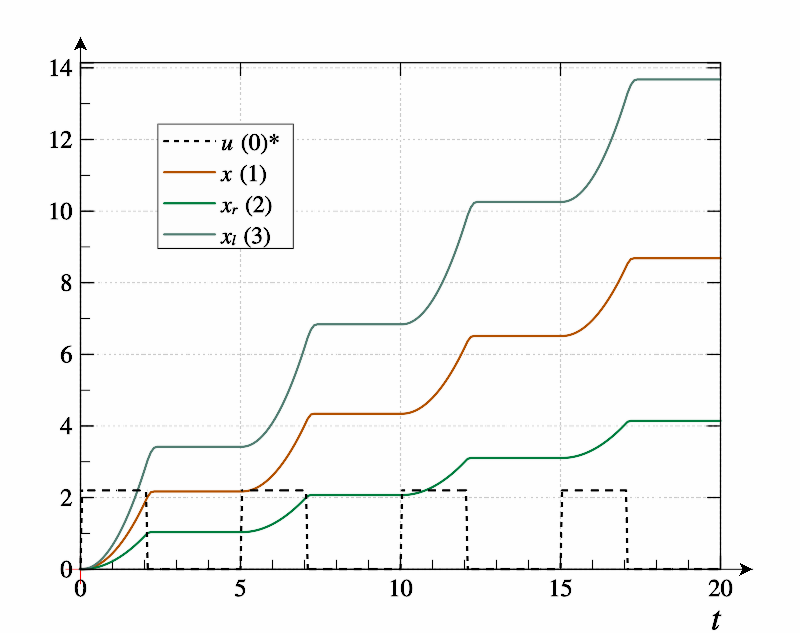
\includegraphics[width=0.5\textwidth]{p/cha/fric/fric_outs1.png}
  }
  \caption{Динаміка трьох моделей виду (\ref{atu:eq:dryfric_sys})}
  \label{atu:f:fric_outs}
\end{figure}

При подальшому моделюванні, в якості сигналу
$u(t)$ використовувався кусочно-лінійний періодичний сигнал,
в якому чергуються ``плато'' і різкі зміни. Вибір такої форми
обумовлений характерними режимами роботи систем позиціювання
електромеханічних пристроїв, для яких вплив сухого тертя є важливим компонентом.

% }}}2

\subsection{Аналіз і вибір критеріїв} % {{{2

Для забезпечення можливості застосування методів ідентифікації, важливе
існування критерію $q(x(t))$, що задовольняє наступним вимогам:

\begin{itemize}

  \item
    чутливість до динаміки моделі і об'єкта;

  \item
    властивість астатизму,
    тобто незалежність від зсуву виходу об'єкта або моделі:
    \( q(x(t)+a ) \approx q( x(t) ) \);

  \item
    достатня стійкість до шумів вимірювання;

  \item
    фізична реалізація.

\end{itemize}

Перші дві вимоги можуть бути досягнуті шляхом обчислення
похідної ---
швидкості зміни вихідних сигналів
\(v = \mathrm{d} \, x (t) / \mathrm{d} \, t \),
і формування критерію ідентифікації на цієї основі.

Однак, при цьому система стає занадто чутливою до шумів
вимірювання. Навіть в тому випадку, коли оцінка похідної
проводиться фізично реалізованими методами, створити
працездатну систему ідентифікації на основі критеріїв
подібного виду практично неможливо.

В роботі \cite{atu_asau11} був запропонований метод синтезу критерію
ідентифікації на основі гістерезисної фільтрації вихідних
сигналів, з подальшим обчисленням похідної. Метод показав свою
працездатність, однак, він вимагає досить точної інформації про
рівень і вигляд шумів --- для налаштування гістерезисного фільтру.
У даній роботі зроблено припущення, що рівень шумів дозволяє створити фільтр, який
подавляє шуми за (як максимум) характерний час реакції системи. Після
фільтра діє реальна ланка, що диференціює. Відповідний вид критерію позначимо як
$q_{dx}$ (рис.~\ref{atu:f:fric_q}).

\begin{figure}[htb!]
\centerline{
  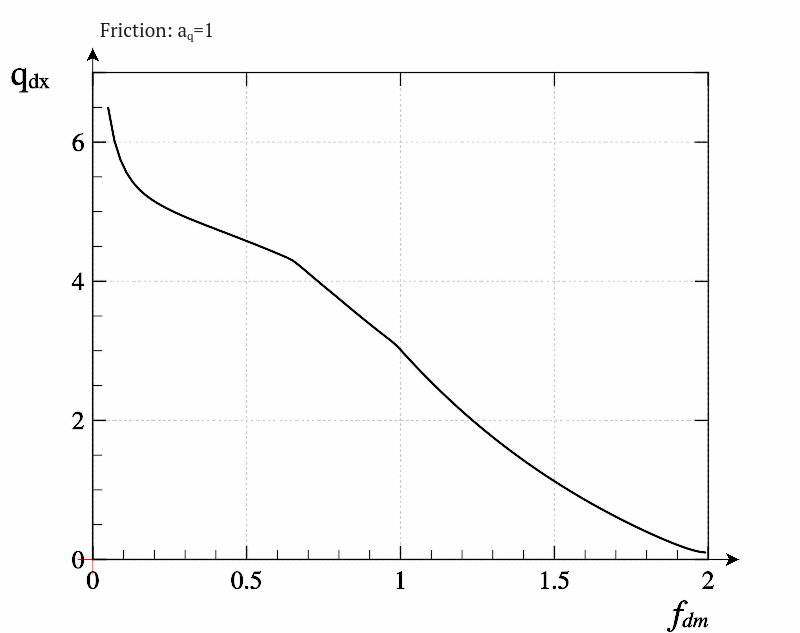
\includegraphics[width=0.60\textwidth]{p/cha/fric/fric_q-p_f_dm_q.png}
}
\caption{Залежність $q_{dx}(f_{dm})$ для системи (\ref{atu:eq:dryfric_sys}) }
\label{atu:f:fric_q}
\end{figure}

Незважаючи на виражену нелінійність в початковій частині
графіка, цей критерій видається цілком прийнятним для задачі
ідентифікації, з огляду на монотонність і обмежений діапазон
похідної. При великих значеннях параметра
$f_{dm}$ сенс цього критерію втрачається, так як відсутня динаміка
системи. При малих значеннях можливості ідентифікації теж
сильно обмежені, так як динаміка системи більше визначається
масою об'єкта, ніж нехтовно малою силою тертя.

% }}}2


\subsection{Тестова задача ідентифікації} % {{{2

Аналогічно вже розглянутим систем визначимо тестове завдання
наступним чином:
\[
  f_{dm}(t) \equiv p_o(t) \in (0.1, 1.5),
\]
%
\begin{equation}
  p_o(t) = p_0 +  U_{p} \sign \sin( \omega_{p} t ),
  \label{atu:eq:fric_po_t_sign}
\end{equation}
%
%
\begin{equation}
  p_o(t) = p_0 +  U_{p} \sin( \omega_{p} t ),
  \label{atu:eq:fric_po_t_sin}
\end{equation}
%
де:
$p_0 = 0.7$, $U_p=0.4$, $\omega_p = \pi / 300$.

Динаміка процесів ідентифікації для системи (\ref{atu:eq:dryfric_sys})
з використанням групи методів ql3rlWvnAAW.$q_\mathrm{dx} $ за умови (\ref{atu:eq:fric_po_t_sign})
представлена на рис.~\ref{atu:f:fric_id_ql3rlWvnAAW_q_dx_sign}.

\begin{figure}[htb!]
  \PicDouble{p/cha/fric/ql3rlWvnAAW/fric_id-p_t_pi_ql3rlWvnAAW_sign.png}{p/cha/fric/ql3rlWvnAAW/fric_id-p_t_p_ql3rlWvnAAW_sign.png}
\caption{
  Процес ідентифікації параметра $f_{dm}$ системи (\ref{atu:eq:dryfric_sys}) групою методів ``ql3rlWvnAAW''
  за умов (\ref{atu:eq:po_t_sign})~(a) і  (\ref{atu:eq:po_t_sin})~(b)
}
\label{atu:f:fric_id_ql3rlWvnAAW_q_dx_sign}
\end{figure}

Для розглянутих умов спостерігається низький рівень збурень
ідентифікованого параметра. Однак, при малих значеннях
$ f_{dm} $ спостерігається помітна статична похибка
ідентифікації. Це пов'язано з тим, що в цій області вплив тертя
стає малим, і критерій втрачає свою адекватність.

Слід зазначити, що при великих значеннях
$ \omega_p $ спостерігається сильний вплив вхідного сигналу, В силу
того, що коли системи нерухомі на одному з ``плато'', в ці моменти
немає можливості розрізнити їх параметри, якой б критерій при
цьому не використовувався.

Результати моделювання при аналогічних умовах, але при
динаміці параметра, заданої (\ref{atu:eq:fric_po_t_sin}), представлені на
рис.~\ref{atu:f:fric_id_ql3rlWvnAAW_q_dx_sin}.

\begin{figure}[htb!]
  \PicDouble{p/cha/fric/ql3rlWvnAAW/fric_id-p_t_pi_ql3rlWvnAAW_sin.png}{p/cha/fric/ql3rlWvnAAW/fric_id-p_t_p_ql3rlWvnAAW_sin.png}
  \caption{Процес ідентифікації параметра ``$f_{dm}$'' системи (\ref{atu:eq:dryfric_sys}) групою методів ql3rlWvnAAW.$q_\mathrm{dx}$ за умовою~(\ref{atu:eq:fric_po_t_sin}): динаміка агентів~(a) та $p_\mathrm{id}$~(b)}
\label{atu:f:fric_id_ql3rlWvnAAW_q_dx_sin}
\end{figure}

За винятком уже згаданої області, в якій критерій перестає
працювати, спостерігається досить низький рівень помилок
ідентифікації. В першу чергу це обумовлено тим, що дана система
не є хаотичною, і проявляє тільки деякі подібні властивості. І
як наслідок, критерій, заснований на фізичних властивостях
системи, дозволяє створити систему ідентифікації з низьким
рівнем помилок.


% }}}2




\subsection{Вплив параметрів системи ідентифікації на похибку ідентифікації для системи} % {{{2

Відносно низький досягнутий рівень похибки ідентифікації для
даної системи дає можливість докладніше дослідити вплив параметрів
системи ідентифікації.


Залежності
$ \overline{e_*} (a_q) $
(рис.~\ref{atu:f:fric_a_q_ql3rlWvnAAW_q_dx}) дозволяють визначити
коректний час усереднення критерію. Менше оптимальне (в сенсі
мінімуму похибки) значення для плавної зміни значення
параметра є очікуваним явищем. Відмінною особливістю даної
системи є те, що мінімальну похибку ідентифікації дозволяє
досягти метод
$ p_{ge} $ координатора пошуку, а метод
$ p_{le} $, який зазвичай показує кращі результати, знаходиться на
другому місці.

% TODO: why?

\begin{figure}[htb!]
  \PicDouble{p/cha/fric/ql3rlWvnAAW/fric_id-p_a_q_sign.png}{p/cha/fric/ql3rlWvnAAW/fric_id-p_a_q_sin.png}
  \caption{Залежності $ \overline{e} (a_q)$ при ідентифікації системи (\ref{atu:eq:dryfric_sys}) групою методів ql3rlWvnAAW.$q_\mathrm{dx} $ при~(\ref{atu:eq:fric_po_t_sign})~(a) і (\ref{atu:eq:fric_po_t_sin})~(b)}
\label{atu:f:fric_a_q_ql3rlWvnAAW_q_dx}
\end{figure}


Залежність помилок ідентифікації від величини коефіцієнта масштабу
$q_\gamma$
(рис.~\ref{atu:f:fric_q_gamma_ql3rlWvnAAW_q_dx})
досить сильно відрізняться від аналогічних для інших систем.

\begin{figure}[htb!]
  \PicDouble{p/cha/fric/ql3rlWvnAAW/fric_id-p_q_gamma_sign.png}{p/cha/fric/ql3rlWvnAAW/fric_id-p_q_gamma_sin.png}
  \caption{Залежності $ \overline{e} (q_\gamma) $ при ідентифікації системи (\ref{atu:eq:dryfric_sys}) групою методів ql3rlWvnAAW.$q_\mathrm{dx} $ при~(\ref{atu:eq:fric_po_t_sign})~(a) і (\ref{atu:eq:fric_po_t_sin})~(b)}
\label{atu:f:fric_q_gamma_ql3rlWvnAAW_q_dx}
\end{figure}

При стрибкоподібних змінах параметра немає характерного
зростання похибки при надмірній чутливості (в обмежених
межах). При цьому існує наявне розділення між результатами
роботи методів координатора пошуку. Методи, які використовують
значення
$ p_e $ від пошукових агентів, показують істотно кращі
результати. Така відмінність досить очевидна, але саме для цієї
системи і цих умов відмінність проявляє собі настільки істотно. У разі плавних
змін параметра відмінність не настільки істотна, але при
недостатній чутливості найкращі результати демонструє метод
$p_{lc}$, що досить несподівано.


На рис.~\ref{atu:f:fric_v_f_ql3rlWvnAAW_q_dx} представлені залежності похибки
ідентифікації від коефіцієнта швидкості пошуку
$v_f$. Вид цих залежностей не проявляє ніяких особливостей. Для
плавних змін параметра виграш від зсуву агентів досягає
800\%, для стрибкоподібних змін --- порядку 20--25\%.

\begin{figure}[htb!]
  \PicDouble{p/cha/fric/ql3rlWvnAAW/fric_id-p_v_f_sign.png}{p/cha/fric/ql3rlWvnAAW/fric_id-p_v_f_sin.png}
  \caption{Залежності $\overline{e}(v_f)$ при ідентифікації системи (\ref{atu:eq:dryfric_sys}) групою методів ql3rlWvnAAW.$q_\mathrm{dx} $ при~(\ref{atu:eq:fric_po_t_sign})~(a) і (\ref{atu:eq:fric_po_t_sin})~(b)}
\label{atu:f:fric_v_f_ql3rlWvnAAW_q_dx}
\end{figure}

Залежності помилок ідентифікації від коефіцієнта
$ k_e $, що визначає рівноважний стан агентів
(рис.~\ref{atu:f:fric_k_e_ql3rlWvnAAW_q_dx}), для даної системи найбільш яскраво
виражені при плавній зміні параметра, що підкреслює користь
від динаміки агентів. Для стрибкоподібної зміни параметрів
динаміка агентів поступається динаміці параметра, і залежності
виражені не настільки істотно.

\begin{figure}[htb!]
  \PicDouble{p/cha/fric/ql3rlWvnAAW/fric_id-p_k_e_sign.png}{p/cha/fric/ql3rlWvnAAW/fric_id-p_k_e_sin.png}
  \caption{Залежності $\overline{e}(k_e)$ при ідентифікації системи (\ref{atu:eq:dryfric_sys}) групою методів ql3rlWvnAAW.$q_\mathrm{dx} $ при~(\ref{atu:eq:fric_po_t_sign})~(a) і (\ref{atu:eq:fric_po_t_sin})~(b)}
  \label{atu:f:fric_k_e_ql3rlWvnAAW_q_dx}
\end{figure}

Залежності похибок ідентифікації від параметра
$k_{nl} $ (рис.~\ref{atu:f:fric_k_nl_ql3rlWvnAAW_q_dx}), який визначає взаємодію між
агентами, при стрибкоподібних змінах параметра не проявляє
істотній залежності. Навпаки, якщо значення
параметра плавно змінюється, існує явно виражений мінімум, відповідний балансу між
практично вільною динамікою агентів (з урахуванням обмежень),
і практично фіксованою сіткою агентів.

\begin{figure}[htb!]
  \PicDouble{p/cha/fric/ql3rlWvnAAW/fric_id-p_k_nl_sign.png}{p/cha/fric/ql3rlWvnAAW/fric_id-p_k_nl_sin.png}
  \caption{Залежності $\overline{e}(k_{nl})$ при ідентифікації системи (\ref{atu:eq:dryfric_sys}) групою методів ql3rlWvnAAW.$q_\mathrm{dx} $ при~(\ref{atu:eq:fric_po_t_sign})~(a) і (\ref{atu:eq:fric_po_t_sin})~(b)}
\label{atu:f:fric_k_nl_ql3rlWvnAAW_q_dx}
\end{figure}


% }}}2

\subsection{Висновки}%{{{2

В цілому, результати моделювання як динаміки системи з силою
сухого тертя, і процесів ідентифікації параметра
$ f_{dm} $ цієї системи, дозволяють зробити наступні висновки:

\begin{itemize}

  \item
    Незважаючи на те, що система не виявляє в розглянутих умовах
    хаотичну динаміку, для її ідентифікації потрібне використання
    спеціального критерію. Це пов'язано з тим, що розглянута система
    має загальну властивість з системами динамічного хаосу --- малі
    зміни параметра або ж вхідного сигналу можуть призводити до
    істотних відмінностей у динаміці.

  \item
    Для даної системи енергетичні критерії, аналогічні застосованим
    в попередніх випадках, виявилися незастосовними. Критерій, хоч і
    заснований на вимірюванні похідною (після фільтрації), виявився
    працездатним. В першу чергу це пов'язано з тим, що в основі були
    покладені фізичні принципи, які для системи з сухим тертям цілком очевидні.

  \item
    Залежності похибки ідентифікації від параметрів системи
    ідентифікації для даної системи виражені досить яскраво, що
    пов'язано з відсутністю справжньої хаотичної динаміки.

\end{itemize}



% }}}2



% }}}1

% vim: fdm=marker foldlevel=1 foldignore="%#" fdc=4 ft=tex
